
\documentclass{beamer}
\usepackage[utf8]{inputenc}
\usepackage[english]{babel}
\usepackage{amsmath}
\usepackage{amssymb}
\usepackage{fancyhdr}
\usepackage{pgfplots}
\usepackage{setspace}
\usepackage{listings}
\pgfplotsset{compat=1.17} 
\usepackage{enumerate}
\usepackage{algorithm}
\usepackage{algpseudocode}
% \geometry{a4paper} % or letter or a5paper or ... etc
% \geometry{landscape} % rotated page geometry
% \usepackage[margin=2cm]{geometry}
\usepackage{minted}
\usepackage[most]{tcolorbox}
\newtcolorbox{tb}[1][]{%
  sharp corners,
  enhanced,
  colback=white,
  height=6cm,
  attach title to upper,
  #1
}

%These setting will make the code areas look Pretty
\lstset{
	escapechar=~,
	numbers=left, 
	%numberstyle=\tiny, 
	stepnumber=1, 
	firstnumber=1,
	%numbersep=5pt,
	language=C,
	% stringstyle=\itfamily,
	%basicstyle=\footnotesize, 
	showstringspaces=false,
	frame=single,
  upquote=true
}

% created 2023-February-5 %
% Theme choice:
% \usetheme{AnnArbor}
\usetheme{focus}
% Title page details: 
\title{CKKS Encoding/Decoding}
\author{Jonathan Parlett}
\date{\today}

\begin{document}

% Title page frame
\begin{frame}
    \titlepage
	\title{CKKS Encoding/Decoding}
	\maketitle
\end{frame}


\begin{frame}{What well cover}
	\begin{itemize}[<+->]
		\item Cyclotomic polynomials and their degrees
		\item A simplified encoding scheme from polynomials with complex coefficients to
		vectors with complex coefficients
		\item The actual encoding scheme from polynomials with integer coefficients
		to vectors of complex coefficients. 
	\end{itemize}
\end{frame}

\begin{frame}{Cyclotomic polynomials}
	\begin{itemize}[<+->]
		\item The $n$-th Cyclotomic polynomial is defined as $\Phi_n(x) = \Pi_{1 \le k \le n | \gcd(k,n) = 1} (x - e^{2i\pi\frac{k}{n}})$
		\item From the constraint that $gcd(k,n) = 1$ you may be able to infer that the degree of the $n$-th
		cyclotomic polynomial is equal to $\rho(n)$ where $\rho$ is Eulers totient function.
		\item This property will be important to consider when you we select a cyclotomic to use for our
		encoding
		\item Another important property of cyclotomics is that there roots are complex conjugates
		of each other. To see this lets look at the 8-th cyclotomic $X^4 + 1$
		\item $\Phi_8(x) = (x - e^{2i \pi \frac{1}{8}})(x - e^{2i \pi \frac{3}{8}})(x - e^{2i \pi \frac{5}{8}})(x - e^{2i \pi \frac{7}{8}})$
	\end{itemize}
\end{frame}

\begin{frame}{Cyclotomic polynomial roots are complex conjugates: Example}
	\begin{itemize}[<+->]
		\item $x^4 + 1 = \Phi_8(x) = (x - e^{2i \pi \frac{1}{8}})(x - e^{2i \pi \frac{3}{8}})(x - e^{2i \pi \frac{5}{8}})(x - e^{2i \pi \frac{7}{8}})$
		\item $ = (x - (\frac{\sqrt{2}}{2} + i\frac{\sqrt{2}}{2}))(x - e^{2i \pi \frac{3}{8}})(x - e^{2i \pi \frac{5}{8}})(x - (\frac{\sqrt{2}}{2} + i\frac{\sqrt{2}}{2}))$
		\item $ = (x - (\frac{\sqrt{2}}{2} + i\frac{\sqrt{2}}{2}))(x - (-\frac{\sqrt{2}}{2} + i\frac{\sqrt{2}}{2}))(x - (-\frac{\sqrt{2}}{2} - i\frac{\sqrt{2}}{2}))(x - (\frac{\sqrt{2}}{2} + i\frac{\sqrt{2}}{2}))$
		\item $ = (x -\frac{\sqrt{2}}{2} - i\frac{\sqrt{2}}{2})(x +\frac{\sqrt{2}}{2} - i\frac{\sqrt{2}}{2})(x +\frac{\sqrt{2}}{2} + i\frac{\sqrt{2}}{2})(x -\frac{\sqrt{2}}{2} - i\frac{\sqrt{2}}{2})$
		\item Grouping real and imaginary parts we can see that the 1st root is the complex of the 4th 
		and the 2nd root is the complex conjugate of the 3rd
		\item $= ([x -\frac{\sqrt{2}}{2}] - i\frac{\sqrt{2}}{2})([x +\frac{\sqrt{2}}{2}] - i\frac{\sqrt{2}}{2})([x +\frac{\sqrt{2}}{2}] + i\frac{\sqrt{2}}{2})([x -\frac{\sqrt{2}}{2}] - i\frac{\sqrt{2}}{2})$
		\item This fact will become important when we are discussing the mapping of polynomials with integer
		coefficients to complex vectors
	\end{itemize}
\end{frame}

\begin{frame}{Simplified encoding scheme}
	\begin{itemize}[<+->]
		\item The input messages in the CKKS scheme are vectors of complex numbers $z \in \mathbb{C}^N$
		where $N$ is called the degree modulus for reasons that will become obvious
		\item All homomorphic operations in the CKKS scheme are performed on polynomials in the ring
		$\frac{\mathbb{Z}[X]}{X^N + 1}$. The homomorphic properties of these operations come as a consequence
		of the properties of these polynomial rings
		\item So the first big thing to understand in order to fully understand CKKS is this encoding
		scheme. How do we get from our complex vectors to our plaintext polynomials
		\item The ultimate is goal to be able to fully understand the map that defines the CKKS encoding algorithm
		$$\sigma^{-1} : \mathbb{C}^N \to \frac{\mathbb{Z}[X]}{X^N + 1}$$
		\item How do they achieve this map from complex vectors to polynomials of integer coefficients

	\end{itemize}
\end{frame}

\begin{frame}{Simplified encoding scheme}
	\begin{itemize}[<+->]
		\item To start we will first understand the simpler map from complex vectors to polynomials with complex
		coefficients 
		$$\sigma^{-1} : \mathbb{C}^N \to \frac{\mathbb{C}[X]}{X^N + 1}$$
		\item The forward map may be easier to consider
		$$\sigma: \frac{\mathbb{C}[X]}{X^N + 1} \to \mathbb{C}^N$$
		% \item This will probably look familiar from previous lectures as this map is really just
		% the $n$-dimensional DFT matrix and its inverse, but lets go through the process regardless
	\end{itemize}
\end{frame}

% \begin{frame}{Simplified encoding scheme}
% 	\begin{itemize}[<+->]
% 		\item First lets notice a few things about the modulus $N$. The ring $\frac{\mathbb{Z}[X]}{X^N + 1}$
% 		is in some way defined by a cyclotomic polynomial of degree $N$.
% 		\item In CKKS they usually consider $N$ to be a power of 2, $N = 2^k$. So we need cyclotomic
% 		polynomial of degree $N = 2^k$.
% 		\item Since as we noted earlier the degree of the $n$-th cyclotomic is equal to $\rho(n)$
% 		it is easy to find a cyclotomic of the appropriate degree as $\rho(2^{k+1}) = 2^k$, since the
% 		only numbers that have a common factor with $2^k$ will be only the even numbers less than $2^k$
% 	\end{itemize}
% \end{frame}

\begin{frame}{Simplified encoding scheme}
	\begin{itemize}[<+->]
		\item Assume we have our cyclotomic of degree $N$. Then to map a polynomial of degree $N$ to
		a vector in $\mathbb{C}^N$ we simply evaluate that polynomial at the $N$ roots our our cyclotomic
		% \item For a single root of unity $\omega$, and a polynomial $P(x)$ we have
		%  $$P(\omega) = a_N\omega^N + a_{N-1}\omega^{N-1} + \cdots + a_0\omega^0 = b_i$$
		\item Our output vector $z \in \mathbb{C}^N$ will be the vector of $b_i$s for all roots of our cyclotomic
		which is ultimately the result of this matrix vector product for $\Phi_8(x) = X^4 + 1$
		\item 
		\begin{center}
			\[
			\begin{pmatrix}
				1 & (e^i\pi/4)^1 &  (e^i\pi/4)^2 &  (e^i\pi/4)^3 & (e^i\pi/4)^4\\  
				1 & (e^i\pi 3/4)^1 &  (e^i\pi 3/4)^2 &  (e^i\pi 3/4)^3 & (e^i\pi 3/4)^4\\  
				1 & (e^i\pi 5/4)^1 &  (e^i\pi 5/4)^2 &  (e^i\pi 5/4)^3 & (e^i\pi 5/4)^4\\  
				1 & (e^i\pi 7/4)^1 &  (e^i\pi 7/4)^2 &  (e^i\pi 7/4)^3 & (e^i\pi 7/4)^4\\  
			\end{pmatrix} \cdot 
			\begin{pmatrix}
				a_0\\
				a_1\\
				a_2\\
				a_3\\
				a_4\\
			\end{pmatrix} =
			\begin{pmatrix}
				z_0\\
				z_1\\
				z_2\\
				z_3\\
				z_4\\
			\end{pmatrix}
			\]
		\end{center}
	\end{itemize}
\end{frame}
\begin{frame}{Simplified encoding scheme}
	\begin{itemize}[<+->]
	\item 
		\begin{center}
			\[
			\begin{pmatrix}
				1 & (e^i\pi/4)^1 &  (e^i\pi/4)^2 &  (e^i\pi/4)^3 & (e^i\pi/4)^4\\  
				1 & (e^i\pi 3/4)^1 &  (e^i\pi 3/4)^2 &  (e^i\pi 3/4)^3 & (e^i\pi 3/4)^4\\  
				1 & (e^i\pi 5/4)^1 &  (e^i\pi 5/4)^2 &  (e^i\pi 5/4)^3 & (e^i\pi 5/4)^4\\  
				1 & (e^i\pi 7/4)^1 &  (e^i\pi 7/4)^2 &  (e^i\pi 7/4)^3 & (e^i\pi 7/4)^4\\  
			\end{pmatrix} \cdot 
			\begin{pmatrix}
				a_0\\
				a_1\\
				a_2\\
				a_3\\
				a_4\\
			\end{pmatrix} =
			\begin{pmatrix}
				z_0\\
				z_1\\
				z_2\\
				z_3\\
				z_4\\
			\end{pmatrix}
			\]
		\end{center}
		\item Here we can see we have the coefficient vector {\bf a} that uniquely determines the polynomial
		and the output vector {\bf z} $\in \mathbb{C}^N$. 
		\item Its clear from this equation that given one we can compute the other
		and since this is a square matrix there is one and only one solution
		\item so it should be intuitive that this transformation defines an isomorphism between $\mathbb{C}^4$ and $\frac{\mathbb{C}[X]}{X^4 + 1}$
	\end{itemize}
\end{frame}

\begin{frame}{Simplified encoding scheme}
	\begin{itemize}[<+->]
		\item At this point we have defined our simplified map and its inverse as essentially the equation we showed
		in the previous slide
		$$\sigma^{-1} : \mathbb{C}^N \to \frac{\mathbb{C}[X]}{X^N + 1}$$
		\item The CKKS map/algorithm $\sigma^{-1} : \mathbb{C}^N \to \frac{\mathbb{Z}[X]}{X^N + 1}$ adds further structure
		in order to place restrictions on this map to ensure that we encode our complex vectors as polynomials with
		integer coefficients only
	\end{itemize}
\end{frame}


\begin{frame}{evaluating polynomials at complex coefficients}
	\begin{itemize}[<+->]
		\item To understand something about the structure of our map well need the fact that evaluating polynomials
		with real coefficients at complex conjugates produces complex conjugates
		\item This should be straight forward if we understand the simpler statement that powers of complex conjugates
		are still complex conjugates
		\item This is simple to show using Euler's formula so we will state it here for clarity
		\end{itemize}
\end{frame}

\begin{frame}{Evaluating polynomials at complex coefficients}
	\begin{itemize}[<+->]
		\item For some $z \in \mathbb{C}$ we have that $z = re^{ix}$ for some $r,x \in \mathbb{R}$
		\item Then its conjugate $\overline{z} = re^{-ix}$ 
		\item 
		\begin{flalign}
			(\overline{z})^n &= (re^{-ix})^n\\
			(\overline{z})^n &= (re^{-nix})\\
			(\overline{z})^n &= (re^{nix})^{-1}\\
			(\overline{z})^n &= (z^n)^{-1}\\
			(\overline{z})^n &= \overline{z^n}\\
		\end{flalign}
		\item Then if we constructed a general polynomial with real coefficients we could use
		this fact to make our conclusion
	\end{itemize}
\end{frame}

\begin{frame}{Evaluating polynomials at complex coefficients:Exampe}
	\begin{itemize}[<+->]
	\item For complex conjugates $2-i$,$2+i$ and polynomial $P(x) = x^2+1$
	\item $P(2-i) = (2-i)^2+1$
	\item $P(2-i) = 4-4i+i^2+1$
	\item $P(2-i) = 4-4i$
	\item Then for the conjugate we have
	\item $P(2+i) = (2+i)^2 + 1$
	\item $P(2+i) = 4+4i +i^2 + 1$
	\item $P(2+i) = 4+4i$
	\item So we can see that they are conjugates
	\end{itemize}
\end{frame}

\begin{frame}{Evaluating polynomials at complex coefficients}
	\begin{itemize}[<+->]
		\item Does this hold for polynomials with complex coefficients?
		\item No to see why just consider that multiplying 2 complex conjugates
		by another complex number does not necessarily produce complex conjugates
		\item Now that we have shown this we can always say for any complex
		$z$ and polynomial with real coefficients $P(x)$, $\overline{P(z)} = P(\overline{z})$
		\item Now lets return to CKKS and our map $\sigma : \frac{\mathbb{C}[X]}{X^N+1} \to \mathbb{C}^N$
	\end{itemize}
\end{frame}

\begin{frame}{Integer Polynomials map to vectors of complex conjugates}
	\begin{itemize}[<+->]
		\item We eventually want to figure out how to map our complex vectors to polynomials with integer coefficients only
		\item So a good place to start would be looking at what integer coefficient polynomials map to under our current transformation $\sigma^{-1}$
		\item Lets first define $\mathcal{R} = \frac{\mathbb{Z}[X]}{X^N + 1}$ to be the space of polynomials with integer coefficients
		\item So more formally our goal is to define the image of $\mathcal{R}$ under our transformation $\sigma$
		denoted $\sigma(\mathcal{R})$
		\item To map some $P(x) \in \mathcal{R}$ to $\mathbb{C}^N$ we evaluate at the roots of our cyclotomic
		\item Recall that the roots of our cyclotomic are complex conjugates of each other. 
	\end{itemize}
\end{frame}


\begin{frame}{Integer Polynomials map to vectors of complex conjugates}
	\begin{itemize}[<+->]
		\item So evaluating our polynomial at the roots of our cyclotomic produces a vector
		of complex conjugates because of the property we showed previously
		\item For a more concrete picture imagine we have the 4 roots of the 8th cyclotomic
		$\Phi_8(x) = X^4 + 1$
		\item 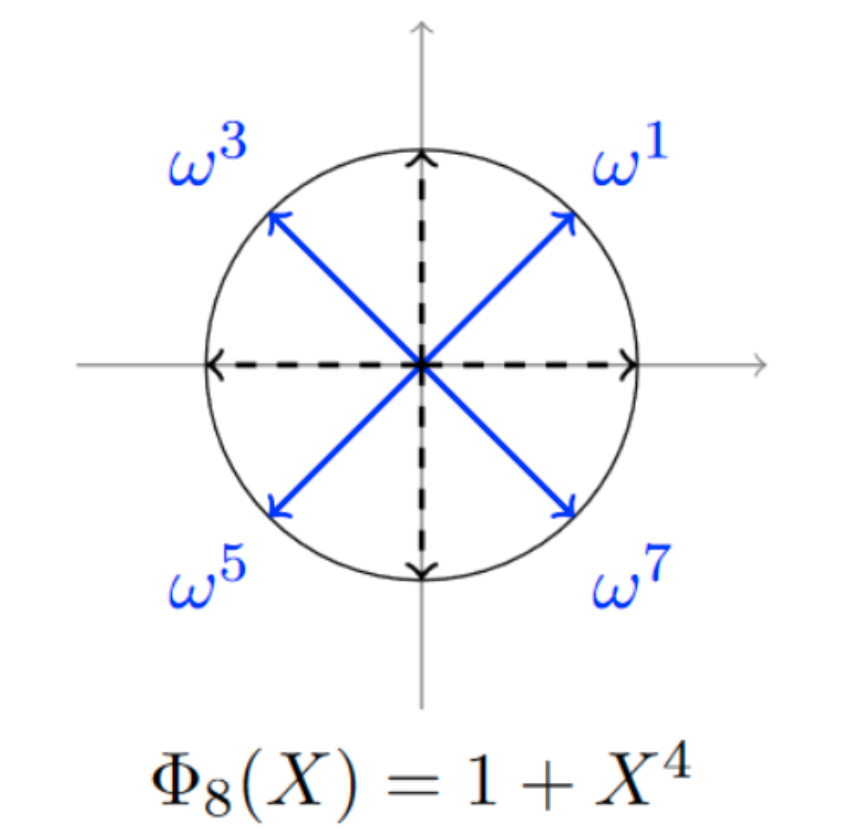
\includegraphics[scale=0.1]{roots.png}
		\item We can see that $\omega^1 = \overline{\omega^7}$ and $\omega^3 = \overline{\omega^5}$
	\end{itemize}
\end{frame}
\begin{frame}{Integer Polynomials map to vectors of complex conjugates}
	\begin{itemize}[<+->]
		\item Take some polynomial $P(x)$ with real coefficients and use it to transform the vector
		$\vec{z} = \langle \omega^1, \omega^3, \omega^5, \omega^7 \rangle$, we can see this satisfies the property $z_i = \overline{z_{4-i}}$
		\item $\langle P(\omega^1), P(\omega^3), P(\omega^5), P(\omega^7) \rangle$
		\item Then this vector is precisely the vector output by our map $\sigma$
		\item $\sigma(P(x)) = \langle P(\omega^1), P(\omega^3), P(\omega^5), P(\omega^7) \rangle$
		\item And since $\overline{P(z)} = P(\overline{z})$ for any complex $z$ we have that
		$P(\omega^1) = \overline{P(\omega^7)}$, and so on
		\item So we have that any polynomial with real coefficients maps to a vector of complex
		conjugates
		\item Based on how we chose to order the conjugates it specifically maps to
		a complex vector $\vec{z} \in \mathbb{C}^N$ s.t $z_i = \overline{z_{N-i}}$
	\end{itemize}
\end{frame}


\begin{frame}{The image of $\mathcal{R}$}
	\begin{itemize}[<+->]
		\item Now consider the set of all complex vectors who's $i$-th coordinates are the complex conjugate of their
		$N-i$-th
		\[\mathbb{H} = \{z \in \mathbb{C}^N | z_i = \overline{z_{N-i}}\} \subset \mathbb{C}^N\]
		\item Now any polynomial with real coefficients maps to a vector in $\mathbb{H}$
		\item So necessarily any polynomial with integer coefficients maps to a vector in $\mathbb{H}$
		\item Now stepping back we can see that we have reached our goal of defining the image of $\mathcal{R}$. Namely it is a subset of
		$\mathbb{H}$
		\[\sigma(\mathcal{R}) \subset \mathbb{H} = \{z \in \mathbb{C}^N | z_i = \overline{z_{N-i}}\} \]
	\end{itemize}
\end{frame}


\begin{frame}{Changing the input space}
	\begin{itemize}[<+->]
		\item Now ultimately we want to be able to map any complex vector to $\sigma(\mathcal{R})$
		\item A first step towards this might be restricting our input vectors to only those complex vectors in $\mathbb{H}$
		\item But how can we do this while preserving the generality of our inputs? We don't want to not be able to encode
		certain messages IE certain vectors in $\mathbb{C}^N$
		\item CKKS solves this problem by instead considering the input space as $\mathbb{C}^{N/2}$ and defining the map
		\[\pi^{-1} : \mathbb{C}^{N/2} \to \mathbb{H}\]
		\item The map itself is rather simplistic. It takes a vector in $\mathbb{C}^{N/2}$ and doubles its size by copying
		all coordinates and conjugating them s.t we have a vector in $\mathbb{H} \subset \mathbb{C}^{N}$
		\item The inverse map $\pi(z) \in \mathbb{C}^{N/2}$ simply cuts the vector in half discarding the 2nd half of conjugates
	\end{itemize}
\end{frame}

\begin{frame}{Changing the input space}
	\begin{itemize}[<+->]
		\item Now by composing these maps we can get from any complex vector to a polynomial with real coefficients
		\[ (\sigma^{-1 } \circ \pi^{-1})(z) : \mathbb{C}^{N/2} \to \frac{\mathbb{R}[x]}{X^N + 1}\]
		\item So almost there, now we just need to narrow our map to get to integer polynomials only. The next step
		is to define a map from $\mathbb{H} \to \sigma(\mathcal{R})$
		\item This process in the paper is described as the discretization of $\pi^{-1}(z)$ to $\sigma(\mathcal{R})$
		\item This is however where I get pretty lost but I will present the theory covered in the paper regardless
	\end{itemize}
\end{frame}

\begin{frame}{Discretization to $\sigma(\mathcal{R})$}
	\begin{itemize}[<+->]
		\item Now $\mathcal{R}$ has a $\mathbb{Z}$-basis $\{1,X,...,X^{N-1}\}$
		\item This is saying that any polynomial in $\mathcal{R}$ can be expressed as a linear combination of the polynomials
		in this $\mathbb{Z}$-basis
		\item Then this basis maps to a rank $N$ ideal lattice $\sigma(\mathcal{R})$ having basis $\{\sigma(1),\sigma(X),...,\sigma(X^{N-1})\}$
		\item This means we have a set of basis vectors for $\sigma(\mathcal{R})$, that constitute a lattice
		\item From my understanding the goal is essentially to compute the closest lattice vector to our given input vector
		thereby transforming our input into a vector that maps to a polynomial in $\mathcal{R}$
	\end{itemize}
\end{frame}

\begin{frame}{Discretization to $\sigma(\mathcal{R})$}
	\begin{itemize}[<+->]
		\item In the paper they do this by first projecting the input vector to the lattice basis, and then via a coordinate
		wise random rounding algorithm fully discretize to a vector in $\sigma(\mathcal{R})$
		\item This operation/map is denoted $\lfloor \cdot \rceil_{\sigma(\mathcal{R})}$
		\item Then we now have a way to get $\mathbb{C}^{N/2} \to \sigma(\mathcal{R})$ via a composition of maps
		\[ \sigma^{-1 } \circ \lfloor \pi^{-1}({\bf z}) \rceil_{\sigma(\mathcal{R})} : \mathbb{C}^{N/2} \to \sigma(\mathcal{R})\]
	\end{itemize}
\end{frame}


\begin{frame}{Scaling to preserve precision}
	\begin{itemize}[<+->]
		\item They also note that the error resulting from rounding may destroy significant figures of the message so they recommend
		multiplying by a scaling factor $\Delta$ before rounding to preserve precision
		\item This changes our current map to
		\[ \sigma^{-1 } \circ \lfloor \Delta \cdot \pi^{-1}({\bf z}) \rceil_{\sigma(\mathcal{R})} : \mathbb{C}^{N/2} \to \sigma(\mathcal{R})\]
	\end{itemize}
\end{frame}


\begin{frame}{The completed encoding algorithm}
	\begin{itemize}[<+->]
		\item Now we can state the CKKS encoding algorithm in full
		\item Take an element $z \in \mathbb{C}^{N/2}$
		\item Expand it to $\pi^{-1}(z) \in \mathbb{H}$
		\item Multiply by $\Delta$ to preserve the desired level of precision
		\item Project to onto our ideal lattice basis via coordinate wise random rounding $\lfloor \Delta \cdot \pi^{-1}({\bf z}) \rceil_{\sigma(\mathcal{R})} \in \sigma(\mathcal{R})$
		\item Finally encode it as a polynomial using $\sigma^{-1}$, $\sigma^{-1 } \circ \lfloor \Delta \cdot \pi^{-1}({\bf z}) \rceil_{\sigma(\mathcal{R})} \in \mathcal{R}$
		\item The decoding procedure is just the inverse of the encoding procedure. We simply apply the inverse maps in reverse order
		to recover the encoded plaintext
	\end{itemize}
\end{frame}

\begin{frame}{The completed encoding algorithm}
	\begin{itemize}[<+->]
		\item That completes our coverage of the encoding and decoding in CKKS. The entire process is summarized succinctly in this
		graphic
		\item 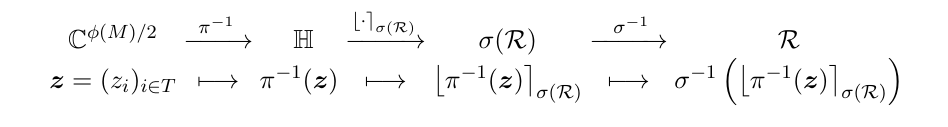
\includegraphics[scale=0.35]{encoding_flow.png}
		\item Thank you for your time!
	\end{itemize}
\end{frame}
\end{document}